\section{概述}
\label{chap:analyze:overview}

%为什么要对丢包的特征进行检测
研究面向VoLTE中主动丢包时间隐通道的检测方法,对改进时间隐通道构建方法,提高抗检测能力有正向促进意义。在VoLTE视频信道中,尤其对于采用了主动丢包的时间隐通道,时间隐通道对IPD分布产生的影响有限。因此,基于IPD的时间隐通道检测方法,忽略了丢包特征,检测效果较差。针对该类时间隐通道,需要设计一种综合的检测方法,结合不同的检测工具对多种分布特征进行检测。

\insertFigure{
	\begin{figure}[htbp]
		\centering
        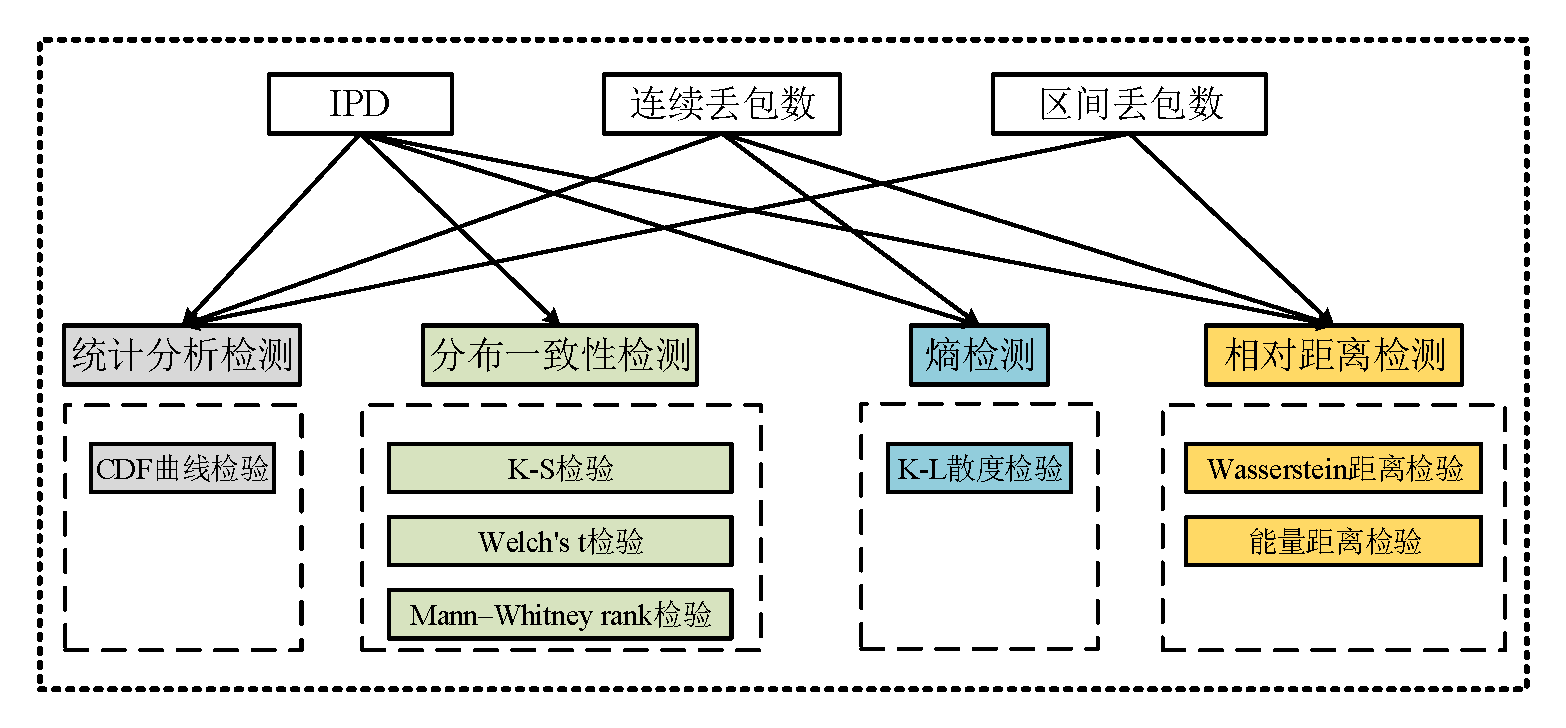
\includegraphics[width=0.9\textwidth]{chapters/chapter3/figures/struct.pdf}
        \caption{面向VoLTE中主动丢包时间隐通道的检测方法结构图}\label{fig:3:struct}
	\end{figure}
}

%检测主要从IPD、丢包特征及突发丢包几个方面展开
丢包事件发生后,产生的影响体现在IPD分布、突发丢包长度,以及区间丢包数分布。如图\nref{fig:3:struct},本检测方法的检测对象包括IPD、突发丢包长度及区间丢包数三种。采用的检测方法分为四类,分别为统计分析检测、分布一致性检测、熵检测及相对距离检测。基于IPD的检测,是时间隐通道的基本检测方法。基于突发丢包长度的检测,重点在于判断不同突发长度的概率,因此适用统计分析检测、熵检测及相对距离检测。基于区间丢包数的检测,重点在于判断分布之间的差异,因此适用统计分析检测及相对距离检测。

%该方法的创新点
该方法的创新点如下:
\begin{itemize}
	\item 除了IPD分布外,同时检测突发丢包长度分布及区间丢包数分布,有效评估了丢包产生的影响;
	\item 检测工具方面,除了基本的CDF检验、K-S检验及K-L散度检验外,同时采用了Welch's t检验、Mann–Whitney rank检验、Wasserstein距离检验及能量距离检验,结合了不同检测工具的优势;
	\item 既能检测基于主动丢包的时间隐通道,同时能够检测基于IPD的时间隐通道。
\end{itemize}

%通过模拟测试,该评估方法具备可行性
为测试该方法的可用性,模拟主动丢包的时间隐通道进行了测试。通过一系列模拟实验,证明该方法在综合了各维度特征后,提升了检测能力,对基于主动丢包的时间隐通道具有良好的分辨能力。